% Figura — Curva CMC conceitual da Fase IV
\begin{figure}[!htb]
\centering
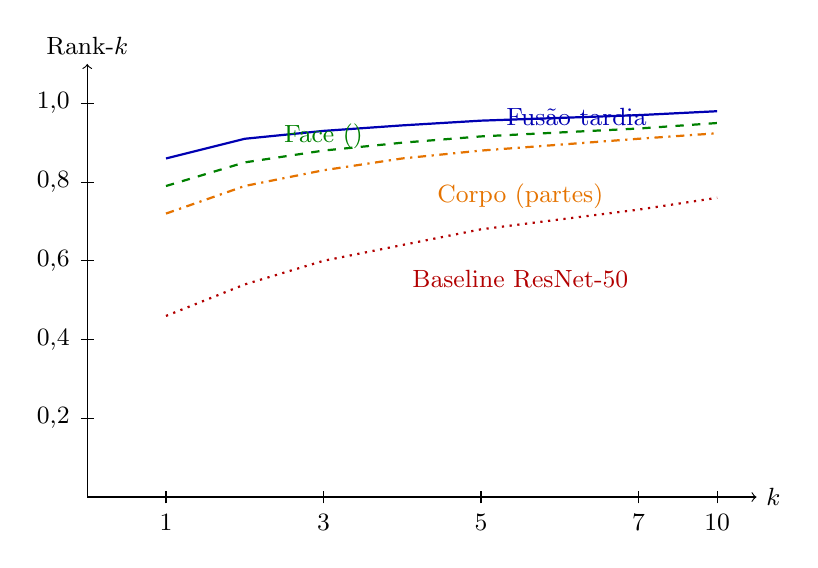
\begin{tikzpicture}[font=\small]
\begin{scope}
  \draw[->] (0,0) -- (8.5,0) node[right]{$k$};
  \draw[->] (0,0) -- (0,5.5) node[above]{Rank-$k$};

  % eixo y
  \foreach \y/\v in {1/0{,}2, 2/0{,}4, 3/0{,}6, 4/0{,}8, 5/1{,}0} {
    \draw (-0.08,\y) -- (0.08,\y);
    \node[left] at (-0.1,\y) {\v};
  }
  % eixo x
  \foreach \x/\v in {1/1, 3/3, 5/5, 7/7, 8/10} {
    \draw (\x,-0.08) -- (\x,0.08);
    \node[below] at (\x,-0.1) {\v};
  }

  % Fusão tardia (azul, melhor)
  \draw[thick, blue!70!black]
    plot coordinates {(1,4.3) (2,4.55) (3,4.65) (4,4.72) (5,4.78) (7,4.85) (8,4.90)};
  \node[blue!70!black, anchor=south west] at (5.2,4.6) {Fusão tardia};

  % Face (verde)
  \draw[thick, green!50!black, dashed]
    plot coordinates {(1,3.95) (2,4.25) (3,4.40) (4,4.50) (5,4.58) (7,4.68) (8,4.75)};
  \node[green!50!black, anchor=south] at (3.0,4.30) {Face (\modeloPetFace)};

  % Corpo (laranja)
  \draw[thick, orange!90!black, dash dot]
    plot coordinates {(1,3.60) (2,3.95) (3,4.15) (4,4.30) (5,4.40) (7,4.55) (8,4.62)};
  \node[orange!90!black, anchor=north] at (5.5,4.10) {Corpo (partes)};

  % Baseline (vermelho)
  \draw[thick, red!70!black, dotted]
    plot coordinates {(1,2.3) (2,2.7) (3,3.0) (4,3.2) (5,3.4) (7,3.65) (8,3.80)};
  \node[red!70!black, anchor=north] at (5.5,3.0) {Baseline ResNet-50};
\end{scope}
\end{tikzpicture}
\caption{Curva CMC conceitual da Fase~IV (regime \emph{closed-set}). \obsfic{traços ilustrativos, a substituir pelas curvas medidas.}}
\label{fig:res-fase4-cmc}
\end{figure}
